% Options for packages loaded elsewhere
\PassOptionsToPackage{unicode}{hyperref}
\PassOptionsToPackage{hyphens}{url}
\PassOptionsToPackage{dvipsnames,svgnames,x11names}{xcolor}
%
\documentclass[
  letterpaper,
  DIV=11,
  numbers=noendperiod]{scrreprt}

\usepackage{amsmath,amssymb}
\usepackage{iftex}
\ifPDFTeX
  \usepackage[T1]{fontenc}
  \usepackage[utf8]{inputenc}
  \usepackage{textcomp} % provide euro and other symbols
\else % if luatex or xetex
  \usepackage{unicode-math}
  \defaultfontfeatures{Scale=MatchLowercase}
  \defaultfontfeatures[\rmfamily]{Ligatures=TeX,Scale=1}
\fi
\usepackage{lmodern}
\ifPDFTeX\else  
    % xetex/luatex font selection
\fi
% Use upquote if available, for straight quotes in verbatim environments
\IfFileExists{upquote.sty}{\usepackage{upquote}}{}
\IfFileExists{microtype.sty}{% use microtype if available
  \usepackage[]{microtype}
  \UseMicrotypeSet[protrusion]{basicmath} % disable protrusion for tt fonts
}{}
\makeatletter
\@ifundefined{KOMAClassName}{% if non-KOMA class
  \IfFileExists{parskip.sty}{%
    \usepackage{parskip}
  }{% else
    \setlength{\parindent}{0pt}
    \setlength{\parskip}{6pt plus 2pt minus 1pt}}
}{% if KOMA class
  \KOMAoptions{parskip=half}}
\makeatother
\usepackage{xcolor}
\setlength{\emergencystretch}{3em} % prevent overfull lines
\setcounter{secnumdepth}{5}
% Make \paragraph and \subparagraph free-standing
\ifx\paragraph\undefined\else
  \let\oldparagraph\paragraph
  \renewcommand{\paragraph}[1]{\oldparagraph{#1}\mbox{}}
\fi
\ifx\subparagraph\undefined\else
  \let\oldsubparagraph\subparagraph
  \renewcommand{\subparagraph}[1]{\oldsubparagraph{#1}\mbox{}}
\fi

\usepackage{color}
\usepackage{fancyvrb}
\newcommand{\VerbBar}{|}
\newcommand{\VERB}{\Verb[commandchars=\\\{\}]}
\DefineVerbatimEnvironment{Highlighting}{Verbatim}{commandchars=\\\{\}}
% Add ',fontsize=\small' for more characters per line
\usepackage{framed}
\definecolor{shadecolor}{RGB}{241,243,245}
\newenvironment{Shaded}{\begin{snugshade}}{\end{snugshade}}
\newcommand{\AlertTok}[1]{\textcolor[rgb]{0.68,0.00,0.00}{#1}}
\newcommand{\AnnotationTok}[1]{\textcolor[rgb]{0.37,0.37,0.37}{#1}}
\newcommand{\AttributeTok}[1]{\textcolor[rgb]{0.40,0.45,0.13}{#1}}
\newcommand{\BaseNTok}[1]{\textcolor[rgb]{0.68,0.00,0.00}{#1}}
\newcommand{\BuiltInTok}[1]{\textcolor[rgb]{0.00,0.23,0.31}{#1}}
\newcommand{\CharTok}[1]{\textcolor[rgb]{0.13,0.47,0.30}{#1}}
\newcommand{\CommentTok}[1]{\textcolor[rgb]{0.37,0.37,0.37}{#1}}
\newcommand{\CommentVarTok}[1]{\textcolor[rgb]{0.37,0.37,0.37}{\textit{#1}}}
\newcommand{\ConstantTok}[1]{\textcolor[rgb]{0.56,0.35,0.01}{#1}}
\newcommand{\ControlFlowTok}[1]{\textcolor[rgb]{0.00,0.23,0.31}{#1}}
\newcommand{\DataTypeTok}[1]{\textcolor[rgb]{0.68,0.00,0.00}{#1}}
\newcommand{\DecValTok}[1]{\textcolor[rgb]{0.68,0.00,0.00}{#1}}
\newcommand{\DocumentationTok}[1]{\textcolor[rgb]{0.37,0.37,0.37}{\textit{#1}}}
\newcommand{\ErrorTok}[1]{\textcolor[rgb]{0.68,0.00,0.00}{#1}}
\newcommand{\ExtensionTok}[1]{\textcolor[rgb]{0.00,0.23,0.31}{#1}}
\newcommand{\FloatTok}[1]{\textcolor[rgb]{0.68,0.00,0.00}{#1}}
\newcommand{\FunctionTok}[1]{\textcolor[rgb]{0.28,0.35,0.67}{#1}}
\newcommand{\ImportTok}[1]{\textcolor[rgb]{0.00,0.46,0.62}{#1}}
\newcommand{\InformationTok}[1]{\textcolor[rgb]{0.37,0.37,0.37}{#1}}
\newcommand{\KeywordTok}[1]{\textcolor[rgb]{0.00,0.23,0.31}{#1}}
\newcommand{\NormalTok}[1]{\textcolor[rgb]{0.00,0.23,0.31}{#1}}
\newcommand{\OperatorTok}[1]{\textcolor[rgb]{0.37,0.37,0.37}{#1}}
\newcommand{\OtherTok}[1]{\textcolor[rgb]{0.00,0.23,0.31}{#1}}
\newcommand{\PreprocessorTok}[1]{\textcolor[rgb]{0.68,0.00,0.00}{#1}}
\newcommand{\RegionMarkerTok}[1]{\textcolor[rgb]{0.00,0.23,0.31}{#1}}
\newcommand{\SpecialCharTok}[1]{\textcolor[rgb]{0.37,0.37,0.37}{#1}}
\newcommand{\SpecialStringTok}[1]{\textcolor[rgb]{0.13,0.47,0.30}{#1}}
\newcommand{\StringTok}[1]{\textcolor[rgb]{0.13,0.47,0.30}{#1}}
\newcommand{\VariableTok}[1]{\textcolor[rgb]{0.07,0.07,0.07}{#1}}
\newcommand{\VerbatimStringTok}[1]{\textcolor[rgb]{0.13,0.47,0.30}{#1}}
\newcommand{\WarningTok}[1]{\textcolor[rgb]{0.37,0.37,0.37}{\textit{#1}}}

\providecommand{\tightlist}{%
  \setlength{\itemsep}{0pt}\setlength{\parskip}{0pt}}\usepackage{longtable,booktabs,array}
\usepackage{calc} % for calculating minipage widths
% Correct order of tables after \paragraph or \subparagraph
\usepackage{etoolbox}
\makeatletter
\patchcmd\longtable{\par}{\if@noskipsec\mbox{}\fi\par}{}{}
\makeatother
% Allow footnotes in longtable head/foot
\IfFileExists{footnotehyper.sty}{\usepackage{footnotehyper}}{\usepackage{footnote}}
\makesavenoteenv{longtable}
\usepackage{graphicx}
\makeatletter
\def\maxwidth{\ifdim\Gin@nat@width>\linewidth\linewidth\else\Gin@nat@width\fi}
\def\maxheight{\ifdim\Gin@nat@height>\textheight\textheight\else\Gin@nat@height\fi}
\makeatother
% Scale images if necessary, so that they will not overflow the page
% margins by default, and it is still possible to overwrite the defaults
% using explicit options in \includegraphics[width, height, ...]{}
\setkeys{Gin}{width=\maxwidth,height=\maxheight,keepaspectratio}
% Set default figure placement to htbp
\makeatletter
\def\fps@figure{htbp}
\makeatother

\KOMAoption{captions}{tableheading}
\makeatletter
\makeatother
\makeatletter
\@ifpackageloaded{bookmark}{}{\usepackage{bookmark}}
\makeatother
\makeatletter
\@ifpackageloaded{caption}{}{\usepackage{caption}}
\AtBeginDocument{%
\ifdefined\contentsname
  \renewcommand*\contentsname{Table of contents}
\else
  \newcommand\contentsname{Table of contents}
\fi
\ifdefined\listfigurename
  \renewcommand*\listfigurename{List of Figures}
\else
  \newcommand\listfigurename{List of Figures}
\fi
\ifdefined\listtablename
  \renewcommand*\listtablename{List of Tables}
\else
  \newcommand\listtablename{List of Tables}
\fi
\ifdefined\figurename
  \renewcommand*\figurename{Figure}
\else
  \newcommand\figurename{Figure}
\fi
\ifdefined\tablename
  \renewcommand*\tablename{Table}
\else
  \newcommand\tablename{Table}
\fi
}
\@ifpackageloaded{float}{}{\usepackage{float}}
\floatstyle{ruled}
\@ifundefined{c@chapter}{\newfloat{codelisting}{h}{lop}}{\newfloat{codelisting}{h}{lop}[chapter]}
\floatname{codelisting}{Listing}
\newcommand*\listoflistings{\listof{codelisting}{List of Listings}}
\makeatother
\makeatletter
\@ifpackageloaded{caption}{}{\usepackage{caption}}
\@ifpackageloaded{subcaption}{}{\usepackage{subcaption}}
\makeatother
\makeatletter
\@ifpackageloaded{tcolorbox}{}{\usepackage[skins,breakable]{tcolorbox}}
\makeatother
\makeatletter
\@ifundefined{shadecolor}{\definecolor{shadecolor}{rgb}{.97, .97, .97}}
\makeatother
\makeatletter
\makeatother
\makeatletter
\makeatother
\ifLuaTeX
  \usepackage{selnolig}  % disable illegal ligatures
\fi
\IfFileExists{bookmark.sty}{\usepackage{bookmark}}{\usepackage{hyperref}}
\IfFileExists{xurl.sty}{\usepackage{xurl}}{} % add URL line breaks if available
\urlstyle{same} % disable monospaced font for URLs
\hypersetup{
  pdftitle={R \& GIS for Geoinformatics},
  pdfauthor={Lika Zhvania},
  colorlinks=true,
  linkcolor={blue},
  filecolor={Maroon},
  citecolor={Blue},
  urlcolor={Blue},
  pdfcreator={LaTeX via pandoc}}

\title{R \& GIS for Geoinformatics}
\author{Lika Zhvania}
\date{}

\begin{document}
\maketitle
\ifdefined\Shaded\renewenvironment{Shaded}{\begin{tcolorbox}[sharp corners, boxrule=0pt, breakable, borderline west={3pt}{0pt}{shadecolor}, enhanced, interior hidden, frame hidden]}{\end{tcolorbox}}\fi

\renewcommand*\contentsname{Table of contents}
{
\hypersetup{linkcolor=}
\setcounter{tocdepth}{2}
\tableofcontents
}
\bookmarksetup{startatroot}

\hypertarget{welcome}{%
\chapter*{Welcome}\label{welcome}}
\addcontentsline{toc}{chapter}{Welcome}

\markboth{Welcome}{Welcome}

\part{Foundations}

\hypertarget{getting-set-up}{%
\chapter{Getting set up}\label{getting-set-up}}

R \& GIS for Geoinformatics (B.Sc.)

\hfill\break

\hypertarget{learning-objectives}{%
\section{Learning objectives}\label{learning-objectives}}

\begin{itemize}
\tightlist
\item
  Create \& organise an RStudio \textbf{Project} and plain \textbf{R
  scripts}
\item
  Install and load R packages (\texttt{tidyverse}, \texttt{sf},
  \texttt{ggplot2})
\item
  Import, explore, summarise, and visualise a dataset
\item
  Open a new \textbf{QGIS} project, set a working folder, and save
  settings
\item
  Add basemaps and sample data; explore the QGIS interface and key
  plugins
\end{itemize}

\begin{center}\rule{0.5\linewidth}{0.5pt}\end{center}

\hypertarget{pre-class-checklist}{%
\section{Pre-class checklist}\label{pre-class-checklist}}

\begin{longtable}[]{@{}ll@{}}
\toprule\noalign{}
Software & Version / link \\
\midrule\noalign{}
\endhead
\bottomrule\noalign{}
\endlastfoot
\textbf{R} & ≥ 4.3 \url{https://cran.r-project.org} \\
\textbf{RStudio Desktop} & Latest \url{https://posit.co/download} \\
\textbf{QGIS} & 3.34 (LTR) \url{https://qgis.org} \\
\textbf{Git} (optional) & ≥ 2.40 \\
\end{longtable}

Create a folder \texttt{geo-course/} somewhere you have write access.
We'll treat this as your \textbf{working directory} for the whole
semester.

\begin{center}\rule{0.5\linewidth}{0.5pt}\end{center}

\hypertarget{part-a---r-basics}{%
\section{Part A - R Basics}\label{part-a---r-basics}}

\hypertarget{create-an-r-script}{%
\subsection{Create an R script}\label{create-an-r-script}}

\begin{enumerate}
\def\labelenumi{\arabic{enumi}.}
\tightlist
\item
  Launch \textbf{RStudio} → \emph{File ▸ New Project ▸ Existing
  Directory} → point to \texttt{geo-course/}.
\item
  \emph{File ▸ New File ▸ R Script} → save as \texttt{week01\_intro.R}.
\item
  At the very top add:
\end{enumerate}

\begin{Shaded}
\begin{Highlighting}[]
\CommentTok{\# week01\_intro.R  {-}{-} your first R commands}
\FunctionTok{print}\NormalTok{(}\StringTok{"Hello, GIS world!"}\NormalTok{)}
\end{Highlighting}
\end{Shaded}

\begin{verbatim}
[1] "Hello, GIS world!"
\end{verbatim}

Tip: The Files pane mirrors your disk. Use New Folder to keep /data,
/scripts, /outputs tidy.

\hypertarget{install-load-libraries}{%
\subsection{Install \& load libraries}\label{install-load-libraries}}

\begin{Shaded}
\begin{Highlighting}[]
\CommentTok{\# Run **once** per machine}
\CommentTok{\#install.packages(c("tidyverse", "ggplot2", "dplyr", "sf"))}
\end{Highlighting}
\end{Shaded}

\begin{Shaded}
\begin{Highlighting}[]
\CommentTok{\# Run in every new R session}
\FunctionTok{library}\NormalTok{(tidyverse)   }\CommentTok{\# loads ggplot2, dplyr, readr, etc.}
\end{Highlighting}
\end{Shaded}

\begin{verbatim}
-- Attaching core tidyverse packages ------------------------ tidyverse 2.0.0 --
v dplyr     1.1.4     v readr     2.1.5
v forcats   1.0.0     v stringr   1.5.1
v ggplot2   3.5.0     v tibble    3.2.1
v lubridate 1.9.3     v tidyr     1.3.1
v purrr     1.0.2     
-- Conflicts ------------------------------------------ tidyverse_conflicts() --
x dplyr::filter() masks stats::filter()
x dplyr::lag()    masks stats::lag()
i Use the conflicted package (<http://conflicted.r-lib.org/>) to force all conflicts to become errors
\end{verbatim}

\begin{Shaded}
\begin{Highlighting}[]
\FunctionTok{library}\NormalTok{(sf)          }\CommentTok{\# spatial data}
\end{Highlighting}
\end{Shaded}

\begin{verbatim}
Linking to GEOS 3.11.2, GDAL 3.8.2, PROJ 9.3.1; sf_use_s2() is TRUE
\end{verbatim}

\hypertarget{core-syntax-refresher}{%
\subsection{Core syntax refresher}\label{core-syntax-refresher}}

\begin{Shaded}
\begin{Highlighting}[]
\CommentTok{\# assigning objects}
\NormalTok{greeting }\OtherTok{\textless{}{-}} \StringTok{"Hello, R!"}
\NormalTok{year     }\OtherTok{\textless{}{-}} \DecValTok{2025}
\NormalTok{is\_spatial }\OtherTok{\textless{}{-}} \ConstantTok{TRUE}
\end{Highlighting}
\end{Shaded}

\begin{Shaded}
\begin{Highlighting}[]
\NormalTok{greeting}
\end{Highlighting}
\end{Shaded}

\begin{verbatim}
[1] "Hello, R!"
\end{verbatim}

\begin{Shaded}
\begin{Highlighting}[]
\NormalTok{year}
\end{Highlighting}
\end{Shaded}

\begin{verbatim}
[1] 2025
\end{verbatim}

\begin{Shaded}
\begin{Highlighting}[]
\NormalTok{is\_spatial}
\end{Highlighting}
\end{Shaded}

\begin{verbatim}
[1] TRUE
\end{verbatim}

\begin{Shaded}
\begin{Highlighting}[]
\CommentTok{\# vectors ⟶ simple arithmetic}
\NormalTok{nums }\OtherTok{\textless{}{-}} \FunctionTok{c}\NormalTok{(}\DecValTok{1}\NormalTok{, }\DecValTok{2}\NormalTok{, }\DecValTok{3}\NormalTok{, }\DecValTok{4}\NormalTok{)}
\FunctionTok{mean}\NormalTok{(nums)}
\end{Highlighting}
\end{Shaded}

\begin{verbatim}
[1] 2.5
\end{verbatim}

\hypertarget{import-a-built-in-data-set}{%
\subsection{Import a built-in data
set}\label{import-a-built-in-data-set}}

\begin{Shaded}
\begin{Highlighting}[]
\FunctionTok{data}\NormalTok{(}\StringTok{"mtcars"}\NormalTok{)   }\CommentTok{\# 32 cars × 11 variables}
\FunctionTok{head}\NormalTok{(mtcars)}
\end{Highlighting}
\end{Shaded}

\begin{verbatim}
                   mpg cyl disp  hp drat    wt  qsec vs am gear carb
Mazda RX4         21.0   6  160 110 3.90 2.620 16.46  0  1    4    4
Mazda RX4 Wag     21.0   6  160 110 3.90 2.875 17.02  0  1    4    4
Datsun 710        22.8   4  108  93 3.85 2.320 18.61  1  1    4    1
Hornet 4 Drive    21.4   6  258 110 3.08 3.215 19.44  1  0    3    1
Hornet Sportabout 18.7   8  360 175 3.15 3.440 17.02  0  0    3    2
Valiant           18.1   6  225 105 2.76 3.460 20.22  1  0    3    1
\end{verbatim}

(Later we'll replace this with real spatial data.)

\hypertarget{basic-data-manipulation}{%
\subsection{Basic data manipulation}\label{basic-data-manipulation}}

\begin{Shaded}
\begin{Highlighting}[]
\NormalTok{mtcars }\SpecialCharTok{|\textgreater{}}
  \FunctionTok{summarise}\NormalTok{(}
    \AttributeTok{cars        =} \FunctionTok{n}\NormalTok{(),}
    \AttributeTok{mean\_mpg    =} \FunctionTok{mean}\NormalTok{(mpg),}
    \AttributeTok{best\_eff    =} \FunctionTok{max}\NormalTok{(mpg)}
\NormalTok{  )}
\end{Highlighting}
\end{Shaded}

\begin{verbatim}
  cars mean_mpg best_eff
1   32 20.09062     33.9
\end{verbatim}

Group by cylinders:

\begin{Shaded}
\begin{Highlighting}[]
\NormalTok{mtcars }\SpecialCharTok{|\textgreater{}}
  \FunctionTok{group\_by}\NormalTok{(cyl) }\SpecialCharTok{|\textgreater{}}
  \FunctionTok{summarise}\NormalTok{(}\FunctionTok{across}\NormalTok{(mpg, }\FunctionTok{list}\NormalTok{(}\AttributeTok{min =}\NormalTok{ min,}
                             \AttributeTok{mean =}\NormalTok{ mean,}
                             \AttributeTok{max =}\NormalTok{ max)))}
\end{Highlighting}
\end{Shaded}

\begin{verbatim}
# A tibble: 3 x 4
    cyl mpg_min mpg_mean mpg_max
  <dbl>   <dbl>    <dbl>   <dbl>
1     4    21.4     26.7    33.9
2     6    17.8     19.7    21.4
3     8    10.4     15.1    19.2
\end{verbatim}

\hypertarget{first-ggplot}{%
\subsection{First ggplot}\label{first-ggplot}}

\begin{Shaded}
\begin{Highlighting}[]
\FunctionTok{ggplot}\NormalTok{(mtcars, }\FunctionTok{aes}\NormalTok{(}\AttributeTok{x =}\NormalTok{ wt, }\AttributeTok{y =}\NormalTok{ mpg)) }\SpecialCharTok{+}
  \FunctionTok{geom\_point}\NormalTok{() }\SpecialCharTok{+}
  \FunctionTok{labs}\NormalTok{(}\AttributeTok{x =} \StringTok{"Weight (1000 lbs)"}\NormalTok{, }\AttributeTok{y =} \StringTok{"Miles / gallon"}\NormalTok{) }\SpecialCharTok{+}
  \FunctionTok{theme\_minimal}\NormalTok{()}
\end{Highlighting}
\end{Shaded}

\begin{figure}[H]

{\centering 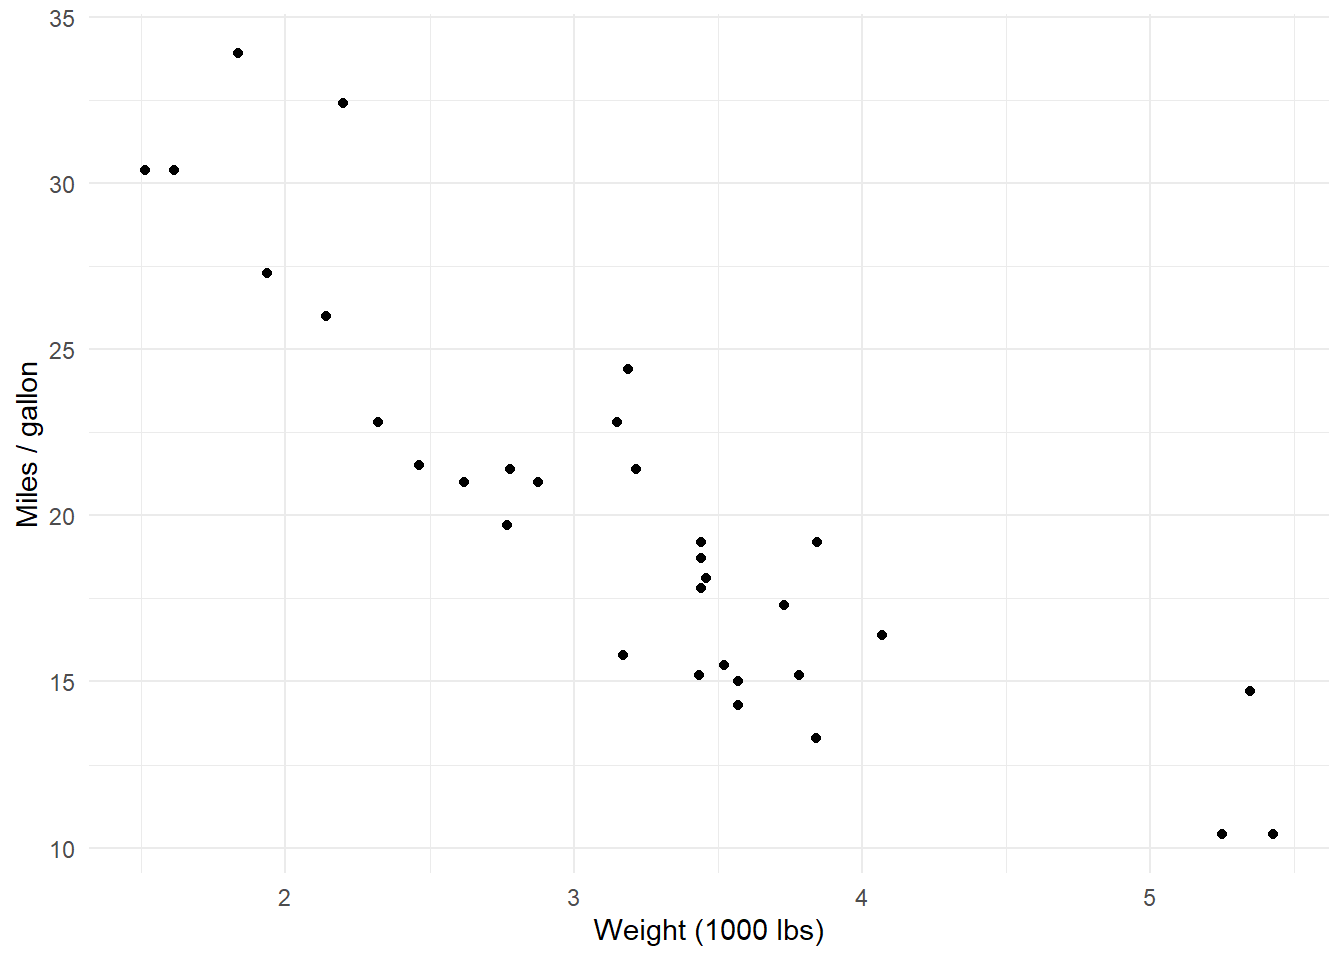
\includegraphics{scripts/week01-getting-setup_files/figure-pdf/unnamed-chunk-10-1.pdf}

}

\end{figure}

Export the plot:

\begin{Shaded}
\begin{Highlighting}[]
\FunctionTok{ggsave}\NormalTok{(}\StringTok{"outputs/mtcars\_wt\_mpg.png"}\NormalTok{, }\AttributeTok{width =} \DecValTok{6}\NormalTok{, }\AttributeTok{height =} \DecValTok{4}\NormalTok{, }\AttributeTok{dpi =} \DecValTok{300}\NormalTok{)}
\end{Highlighting}
\end{Shaded}

\hypertarget{part-b---qgis-basics}{%
\section{Part B - QGIS Basics}\label{part-b---qgis-basics}}

\hypertarget{create-save-a-qgis-project}{%
\subsection{Create \& save a QGIS
project}\label{create-save-a-qgis-project}}

\begin{enumerate}
\def\labelenumi{\arabic{enumi}.}
\tightlist
\item
  Open QGIS 3.34 → Project ▸ New
\item
  Project ▸ Properties ▸ General → set Project home to your geo-course/
  folder.
\item
  Project ▸ Save → week01\_intro.qgz.
\end{enumerate}

This keeps relative paths identical on any PC.

\hypertarget{tour-of-the-interface}{%
\subsection{Tour of the interface}\label{tour-of-the-interface}}

\begin{itemize}
\tightlist
\item
  Browser Panel -- navigate to / drag files
\item
  Layers Panel -- toggle visibility, styling, grouping
\item
  Map Canvas -- the main view
\item
  Processing Toolbox -- scripts \& analysis tools
\item
  Top menus: Vector, Raster, Plugins \ldots{}
\end{itemize}

\hypertarget{add-basemaps-xyz-tiles}{%
\subsection{Add basemaps (XYZ Tiles)}\label{add-basemaps-xyz-tiles}}

Follow the second method in the blog post
https://opengislab.com/\ldots/add-basemaps-in-qgis-30 --- add
QuickMapServices:

\begin{enumerate}
\def\labelenumi{\arabic{enumi}.}
\tightlist
\item
  Plugins ▸ Manage and Install Plugins → search QuickMapServices →
  Install.
\item
  Web ▸ QuickMapServices ▸ Settings ▸ More services → Get contributed
  pack.
\item
  Web ▸ QuickMapServices ▸ OSM ▸ OSM Standard (or any favourite
  basemap).
\end{enumerate}

\hypertarget{load-sample-vector-data}{%
\subsection{Load sample vector data}\label{load-sample-vector-data}}

Grab the Natural Earth admin-0 countries shapefile (≈ 10 MB): * Layer ▸
Add Layer ▸ Add Vector Layer → Protocol → URL:
https://www.naturalearthdata.com/http//www.naturalearthdata.com/download/50m/cultural/ne\_50m\_admin\_0\_countries.zip
Geometry column = the\_geom → Add

Style polygons quickly via Layer Styling ▸ single symbol.

\hypertarget{key-plugins-to-know}{%
\subsection{Key plugins to know}\label{key-plugins-to-know}}

Plugin \textbar{} Why it matters QuickMapServices \textbar{} instant
basemaps QuickOSM \textbar{} download OSM features by query Processing R
Provider \textbar{} run R scripts from within QGIS OpenLayers Plugin
(legacy) \textbar{} alternative basemaps Geometry by Expression
\textbar{} attribute-driven geometry edits

Install via Plugins dialog as needed.

\hypertarget{r-basics}{%
\chapter{R basics}\label{r-basics}}

\hypertarget{quarto}{%
\section{Quarto}\label{quarto}}

Quarto enables you to weave together content and executable code into a
finished document. To learn more about Quarto see
\url{https://quarto.org}.

\hypertarget{running-code}{%
\section{Running Code}\label{running-code}}

When you click the \textbf{Render} button a document will be generated
that includes both content and the output of embedded code. You can
embed code like this:

\begin{Shaded}
\begin{Highlighting}[]
\DecValTok{1} \SpecialCharTok{+} \DecValTok{1}
\end{Highlighting}
\end{Shaded}

\begin{verbatim}
[1] 2
\end{verbatim}

You can add options to executable code like this

\begin{verbatim}
[1] 4
\end{verbatim}

The \texttt{echo:\ false} option disables the printing of code (only
output is displayed).

\hypertarget{data-wrangling-101}{%
\chapter{Data wrangling 101}\label{data-wrangling-101}}

\hypertarget{quarto-1}{%
\section{Quarto}\label{quarto-1}}

Quarto enables you to weave together content and executable code into a
finished document. To learn more about Quarto see
\url{https://quarto.org}.

\hypertarget{running-code-1}{%
\section{Running Code}\label{running-code-1}}

When you click the \textbf{Render} button a document will be generated
that includes both content and the output of embedded code. You can
embed code like this:

\begin{Shaded}
\begin{Highlighting}[]
\DecValTok{1} \SpecialCharTok{+} \DecValTok{1}
\end{Highlighting}
\end{Shaded}

\begin{verbatim}
[1] 2
\end{verbatim}

You can add options to executable code like this

\begin{verbatim}
[1] 4
\end{verbatim}

The \texttt{echo:\ false} option disables the printing of code (only
output is displayed).

\hypertarget{spatial-data-foundations}{%
\chapter{Spatial data foundations}\label{spatial-data-foundations}}

\hypertarget{quarto-2}{%
\section{Quarto}\label{quarto-2}}

Quarto enables you to weave together content and executable code into a
finished document. To learn more about Quarto see
\url{https://quarto.org}.

\hypertarget{running-code-2}{%
\section{Running Code}\label{running-code-2}}

When you click the \textbf{Render} button a document will be generated
that includes both content and the output of embedded code. You can
embed code like this:

\begin{Shaded}
\begin{Highlighting}[]
\DecValTok{1} \SpecialCharTok{+} \DecValTok{1}
\end{Highlighting}
\end{Shaded}

\begin{verbatim}
[1] 2
\end{verbatim}

You can add options to executable code like this

\begin{verbatim}
[1] 4
\end{verbatim}

The \texttt{echo:\ false} option disables the printing of code (only
output is displayed).

\hypertarget{vector-operations-in-r}{%
\chapter{Vector operations in R}\label{vector-operations-in-r}}

\hypertarget{quarto-3}{%
\section{Quarto}\label{quarto-3}}

Quarto enables you to weave together content and executable code into a
finished document. To learn more about Quarto see
\url{https://quarto.org}.

\hypertarget{running-code-3}{%
\section{Running Code}\label{running-code-3}}

When you click the \textbf{Render} button a document will be generated
that includes both content and the output of embedded code. You can
embed code like this:

\begin{Shaded}
\begin{Highlighting}[]
\DecValTok{1} \SpecialCharTok{+} \DecValTok{1}
\end{Highlighting}
\end{Shaded}

\begin{verbatim}
[1] 2
\end{verbatim}

You can add options to executable code like this

\begin{verbatim}
[1] 4
\end{verbatim}

The \texttt{echo:\ false} option disables the printing of code (only
output is displayed).

\hypertarget{raster-essentials}{%
\chapter{Raster essentials}\label{raster-essentials}}

\hypertarget{quarto-4}{%
\section{Quarto}\label{quarto-4}}

Quarto enables you to weave together content and executable code into a
finished document. To learn more about Quarto see
\url{https://quarto.org}.

\hypertarget{running-code-4}{%
\section{Running Code}\label{running-code-4}}

When you click the \textbf{Render} button a document will be generated
that includes both content and the output of embedded code. You can
embed code like this:

\begin{Shaded}
\begin{Highlighting}[]
\DecValTok{1} \SpecialCharTok{+} \DecValTok{1}
\end{Highlighting}
\end{Shaded}

\begin{verbatim}
[1] 2
\end{verbatim}

You can add options to executable code like this

\begin{verbatim}
[1] 4
\end{verbatim}

The \texttt{echo:\ false} option disables the printing of code (only
output is displayed).

\part{Spatial Analysis}

\hypertarget{bridging-r-qgis}{%
\chapter{Bridging R ↔ QGIS}\label{bridging-r-qgis}}

\hypertarget{quarto-5}{%
\section{Quarto}\label{quarto-5}}

Quarto enables you to weave together content and executable code into a
finished document. To learn more about Quarto see
\url{https://quarto.org}.

\hypertarget{running-code-5}{%
\section{Running Code}\label{running-code-5}}

When you click the \textbf{Render} button a document will be generated
that includes both content and the output of embedded code. You can
embed code like this:

\begin{Shaded}
\begin{Highlighting}[]
\DecValTok{1} \SpecialCharTok{+} \DecValTok{1}
\end{Highlighting}
\end{Shaded}

\begin{verbatim}
[1] 2
\end{verbatim}

You can add options to executable code like this

\begin{verbatim}
[1] 4
\end{verbatim}

The \texttt{echo:\ false} option disables the printing of code (only
output is displayed).

\hypertarget{exploratory-spatial-data-analysis-esda}{%
\chapter{Exploratory spatial data analysis
(ESDA)}\label{exploratory-spatial-data-analysis-esda}}

\hypertarget{quarto-6}{%
\section{Quarto}\label{quarto-6}}

Quarto enables you to weave together content and executable code into a
finished document. To learn more about Quarto see
\url{https://quarto.org}.

\hypertarget{running-code-6}{%
\section{Running Code}\label{running-code-6}}

When you click the \textbf{Render} button a document will be generated
that includes both content and the output of embedded code. You can
embed code like this:

\begin{Shaded}
\begin{Highlighting}[]
\DecValTok{1} \SpecialCharTok{+} \DecValTok{1}
\end{Highlighting}
\end{Shaded}

\begin{verbatim}
[1] 2
\end{verbatim}

You can add options to executable code like this

\begin{verbatim}
[1] 4
\end{verbatim}

The \texttt{echo:\ false} option disables the printing of code (only
output is displayed).

\hypertarget{surface-modelling}{%
\chapter{Surface modelling}\label{surface-modelling}}

\hypertarget{quarto-7}{%
\section{Quarto}\label{quarto-7}}

Quarto enables you to weave together content and executable code into a
finished document. To learn more about Quarto see
\url{https://quarto.org}.

\hypertarget{running-code-7}{%
\section{Running Code}\label{running-code-7}}

When you click the \textbf{Render} button a document will be generated
that includes both content and the output of embedded code. You can
embed code like this:

\begin{Shaded}
\begin{Highlighting}[]
\DecValTok{1} \SpecialCharTok{+} \DecValTok{1}
\end{Highlighting}
\end{Shaded}

\begin{verbatim}
[1] 2
\end{verbatim}

You can add options to executable code like this

\begin{verbatim}
[1] 4
\end{verbatim}

The \texttt{echo:\ false} option disables the printing of code (only
output is displayed).

\hypertarget{network-accessibility-analysis}{%
\chapter{Network \& Accessibility
Analysis}\label{network-accessibility-analysis}}

\hypertarget{quarto-8}{%
\section{Quarto}\label{quarto-8}}

Quarto enables you to weave together content and executable code into a
finished document. To learn more about Quarto see
\url{https://quarto.org}.

\hypertarget{running-code-8}{%
\section{Running Code}\label{running-code-8}}

When you click the \textbf{Render} button a document will be generated
that includes both content and the output of embedded code. You can
embed code like this:

\begin{Shaded}
\begin{Highlighting}[]
\DecValTok{1} \SpecialCharTok{+} \DecValTok{1}
\end{Highlighting}
\end{Shaded}

\begin{verbatim}
[1] 2
\end{verbatim}

You can add options to executable code like this

\begin{verbatim}
[1] 4
\end{verbatim}

The \texttt{echo:\ false} option disables the printing of code (only
output is displayed).

\part{Workflow \& Communication}

\hypertarget{automation-reproducibility}{%
\chapter{Automation \&
reproducibility}\label{automation-reproducibility}}

\hypertarget{quarto-9}{%
\section{Quarto}\label{quarto-9}}

Quarto enables you to weave together content and executable code into a
finished document. To learn more about Quarto see
\url{https://quarto.org}.

\hypertarget{running-code-9}{%
\section{Running Code}\label{running-code-9}}

When you click the \textbf{Render} button a document will be generated
that includes both content and the output of embedded code. You can
embed code like this:

\begin{Shaded}
\begin{Highlighting}[]
\DecValTok{1} \SpecialCharTok{+} \DecValTok{1}
\end{Highlighting}
\end{Shaded}

\begin{verbatim}
[1] 2
\end{verbatim}

You can add options to executable code like this

\begin{verbatim}
[1] 4
\end{verbatim}

The \texttt{echo:\ false} option disables the printing of code (only
output is displayed).

\hypertarget{communicating-results}{%
\chapter{Communicating results}\label{communicating-results}}

\hypertarget{quarto-10}{%
\section{Quarto}\label{quarto-10}}

Quarto enables you to weave together content and executable code into a
finished document. To learn more about Quarto see
\url{https://quarto.org}.

\hypertarget{running-code-10}{%
\section{Running Code}\label{running-code-10}}

When you click the \textbf{Render} button a document will be generated
that includes both content and the output of embedded code. You can
embed code like this:

\begin{Shaded}
\begin{Highlighting}[]
\DecValTok{1} \SpecialCharTok{+} \DecValTok{1}
\end{Highlighting}
\end{Shaded}

\begin{verbatim}
[1] 2
\end{verbatim}

You can add options to executable code like this

\begin{verbatim}
[1] 4
\end{verbatim}

The \texttt{echo:\ false} option disables the printing of code (only
output is displayed).

\part{Assignments}

\hypertarget{overview}{%
\chapter*{Overview}\label{overview}}
\addcontentsline{toc}{chapter}{Overview}

\markboth{Overview}{Overview}

This module uses \textbf{two formative assignments} plus a
\textbf{summative final project}:

\begin{longtable}[]{@{}
  >{\raggedright\arraybackslash}p{(\columnwidth - 6\tabcolsep) * \real{0.3481}}
  >{\raggedright\arraybackslash}p{(\columnwidth - 6\tabcolsep) * \real{0.0963}}
  >{\raggedright\arraybackslash}p{(\columnwidth - 6\tabcolsep) * \real{0.0593}}
  >{\raggedright\arraybackslash}p{(\columnwidth - 6\tabcolsep) * \real{0.4963}}@{}}
\toprule\noalign{}
\begin{minipage}[b]{\linewidth}\raggedright
Item
\end{minipage} & \begin{minipage}[b]{\linewidth}\raggedright
When
\end{minipage} & \begin{minipage}[b]{\linewidth}\raggedright
Weight
\end{minipage} & \begin{minipage}[b]{\linewidth}\raggedright
Purpose
\end{minipage} \\
\midrule\noalign{}
\endhead
\bottomrule\noalign{}
\endlastfoot
\textbf{Assignment 1 -- Data Wrangling \& Basic Map} & due Week 7 & 15
\% & Check grasp of tidy data, joins, simple cartography. \\
\textbf{Assignment 2 -- Mini Spatial Model} & due Week 10 & 25 \% &
Apply vector analysis or accessibility workflow to a new dataset. \\
\textbf{Final Project} & exam week & 60 \% & End-to-end case study
integrating R \& QGIS with written report. \\
\end{longtable}

\emph{Late policy, submission format, and marking rubric follow below
\ldots{}}

\hypertarget{assignment-1-data-wrangling}{%
\chapter*{Assignment 1: Data
Wrangling}\label{assignment-1-data-wrangling}}
\addcontentsline{toc}{chapter}{Assignment 1: Data Wrangling}

\markboth{Assignment 1: Data Wrangling}{Assignment 1: Data Wrangling}

\hypertarget{assignment-2-mini-model}{%
\chapter*{Assignment 2: Mini Model}\label{assignment-2-mini-model}}
\addcontentsline{toc}{chapter}{Assignment 2: Mini Model}

\markboth{Assignment 2: Mini Model}{Assignment 2: Mini Model}

\hypertarget{assignment-3-final-project}{%
\chapter*{Assignment 3: Final
Project}\label{assignment-3-final-project}}
\addcontentsline{toc}{chapter}{Assignment 3: Final Project}

\markboth{Assignment 3: Final Project}{Assignment 3: Final Project}



\end{document}
